\documentclass[12pt,a4paper]{report}

% ============================================================================
% PACKAGES & TYPOGRAPHY
% ============================================================================
\usepackage[utf8]{inputenc}
\usepackage[T1]{fontenc}
\usepackage{lmodern}
\usepackage[margin=1in]{geometry}
\usepackage{setspace}
\usepackage{microtype}
\usepackage{amsmath,amssymb,amsfonts,bm}
\usepackage{graphicx}
\usepackage{booktabs}
\usepackage{longtable}
\usepackage{array}
\usepackage{multirow}
\usepackage{tabularx}
\usepackage{xcolor}
\usepackage{colortbl}
\usepackage{enumitem}
\usepackage{caption}
\usepackage{subcaption}
\usepackage{float}
\usepackage{fancyhdr}
\usepackage{titlesec}
\usepackage[numbers,sort&compress]{natbib}
\usepackage{hyperref}

% ============================================================================
% COLOR PALETTE & HYPERREF CONFIGURATION
% ============================================================================
\definecolor{navyblue}{HTML}{1D3557}
\definecolor{steel}{HTML}{457B9D}
\definecolor{tealgreen}{HTML}{2A9D8F}
\definecolor{crimson}{HTML}{E63946}
\definecolor{slate}{HTML}{475569}
\definecolor{rowgray}{HTML}{F8FAFC}

\hypersetup{
    colorlinks=true,
    linkcolor=navyblue,
    citecolor=tealgreen,
    urlcolor=steel,
    pdftitle={CardioCare AI: An Interpretable, Cost-Sensitive Heart Disease Prediction and Clinical Decision Support System},
    pdfauthor={},
    pdfsubject={}
}

\captionsetup{
    font=small,
    labelfont={bf,color=navyblue},
    margin=10pt
}

% Header and Footer Styling (Concise running titles to prevent header overlap)
\setlength{\headheight}{15pt}
\pagestyle{fancy}
\fancyhf{}
\renewcommand{\chaptermark}[1]{\markboth{Chapter \thechapter: #1}{}}
\renewcommand{\sectionmark}[1]{}
\fancyhead[L]{\footnotesize\textcolor{slate}{\textit{CardioCare AI --- Undergraduate Thesis}}}
\fancyhead[R]{\footnotesize\textcolor{slate}{\nouppercase{\leftmark}}}
\fancyfoot[C]{\thepage}
\renewcommand{\headrulewidth}{0.4pt}

% Chapter & Section Title Styling
\titleformat{\chapter}[display]
  {\normalfont\huge\bfseries\color{navyblue}}
  {\chaptertitlename\ \thechapter}{14pt}{\Huge}
\titlespacing*{\chapter}{0pt}{-15pt}{25pt}

\titleformat{\section}
  {\normalfont\Large\bfseries\color{navyblue}}
  {\thesection}{1em}{}

\titleformat{\subsection}
  {\normalfont\large\bfseries\color{steel}}
  {\thesubsection}{1em}{}

\onehalfspacing

\begin{document}

% ============================================================================
% TITLE PAGE
% ============================================================================
\pagenumbering{gobble}
\begin{titlepage}
    \centering
    \vspace*{0.8cm}
    {\scshape\Large Undergraduate Final Year Thesis \& Capstone Report \par}
    \vspace{0.6cm}
    \textcolor{navyblue}{\rule{\linewidth}{1.5pt}}\\[0.4cm]
    {\huge\bfseries\textcolor{navyblue}{CARDIOCARE AI: AN INTERPRETABLE, COST-SENSITIVE HEART DISEASE PREDICTION AND ACTIONABLE CLINICAL DECISION SUPPORT SYSTEM}\par}
    \vspace{0.2cm}
    \textcolor{navyblue}{\rule{\linewidth}{1.5pt}}\\[1.0cm]

    {\Large\itshape Bridging the Gap Between Traditional Epidemiological Risk Scoring, Academic Machine Learning, and Bedside Clinical Utility\par}
    \vspace{1.6cm}

    \begin{tabular}{rl}
        \textbf{Author / Candidate:} &  \\[0.25cm]
        \textbf{Degree Program:} & \\[0.25cm]
        \textbf{Research Domain:} & \\[0.25cm]
        \textbf{Code Repository:} & \texttt{cardiocare-ai} (Python, Scikit-Learn, SHAP, Streamlit) \\[0.25cm]
        \textbf{Date of Submission:} & October 2026
    \end{tabular}

    \vfill

    \begin{minipage}{0.92\textwidth}
        \footnotesize\textcolor{slate}{
        \textbf{Thesis Defense Highlights:} This thesis specifically addresses the foundational question posed by academic examination committees: \emph{``What was done previously, and what is new in this project?''} We identify five critical methodological and clinical flaws in prior work---including target label polarity inversion and 723 duplicate records in public UCI Heart Disease exports, absence of clinical Framingham baseline comparisons, naive symmetric $\tau=0.50$ decision thresholding, misaligned black-box feature attributions, and passive non-actionable diagnoses---and resolve each with rigorous mathematical formulations and empirical validation.}
    \end{minipage}
    \vspace{0.6cm}
\end{titlepage}

% ============================================================================
% FRONT MATTER
% ============================================================================
\clearpage
\pagenumbering{roman}

\chapter*{Abstract}
\markboth{Abstract}{}
\addcontentsline{toc}{chapter}{Abstract}

Cardiovascular diseases (CVDs) remain the leading cause of global mortality, accounting for approximately 17.9 million deaths annually according to the World Health Organization (WHO). In hospital triage and preventive cardiology, risk stratification has historically relied on multivariable parametric heuristics---most notably the Framingham 10-Year Coronary Risk Score (FRS) and the American College of Cardiology / American Heart Association (ACC/AHA) Pooled Cohort Equations. While clinically accessible, these legacy scoring systems rely on rigid linear assumptions, omit exercise electrocardiogram (ECG) and fluoroscopic biomarkers, and exhibit poor sensitivity on acute symptomatic cohorts. Conversely, conventional academic machine learning (ML) projects on the benchmark UCI Heart Disease dataset suffer from five pervasive flaws: (1) unexamined target polarity inversion and 723 duplicate patient records across the 1,025-row multi-center CSV export that cause severe train-test data leakage; (2) evaluation in isolation from real clinical baseline scores; (3) reliance on an arbitrary symmetric $\tau=0.50$ classification threshold that equates fatal False Negatives with benign False Positives; (4) opaque ``black-box'' inference or misaligned feature attribution; and (5) passive diagnostic labeling devoid of actionable therapeutic guidance.

This undergraduate thesis designs, implements, validates, and deploys \textbf{CardioCare AI}, an end-to-end, interpretable, and cost-sensitive clinical decision support system (CDSS). First, we implement automated physiological polarity verification to canonicalize the angiographic disease target ($>50\%$ luminal stenosis) and establish a \textbf{dual-regime evaluation protocol} comparing the standard 1,025-record multi-center benchmark ($N_{\text{test}}=205$) against a strictly deduplicated, patient-disjoint cohort ($N=302$ unique patients, $N_{\text{test}}=61$). Across five supervised learning paradigms---Logistic Regression, Decision Tree, Random Forest, Support Vector Machine (SVM), and Gradient Boosted Decision Trees (GBM)---we demonstrate that GBM achieves \textbf{97.07\% accuracy, 100.00\% sensitivity, 0.9940 ROC-AUC, and 0.0280 Brier calibration score} on the multi-center benchmark, while SVM and Random Forest achieve \textbf{83.61\% and 81.97\% accuracy (0.8853 ROC-AUC)} under strict patient-disjoint deduplication, quantifying the exact $+13.5\%$ to $+15.1\%$ optimistic accuracy inflation present in prior literature.

Second, we implement the standardized adult Framingham 10-Year Coronary Risk Score directly within the evaluation suite, proving that ML ensembles significantly outperform traditional clinical scoring (\textbf{97.07\% vs.\ 61.95\% accuracy; 0.9940 vs.\ 0.6559 ROC-AUC; McNemar's $p = 9.44 \times 10^{-15}$} on the benchmark cohort, and \textbf{0.8853 vs.\ 0.6402 ROC-AUC; McNemar's $p = 0.0123$} on the strict deduplicated cohort). Third, we formulate an asymmetric clinical penalty function ($C_{\text{FN}} = 5.0 \cdot C_{\text{FP}}$) optimized via leakage-free 5-fold out-of-fold (OOF) cross-validation on the training partition ($\tau^* = 0.20$), reducing clinical penalty cost by \textbf{38.9\% for GBM} and \textbf{53.7\% for Random Forest}. Fourth, we integrate ColumnTransformer-aligned cooperative game-theoretic \textbf{TreeSHAP} explainability to generate individualized waterfall plots and global population rankings. Fifth, we engineer a three-tier \textbf{Actionable ``What-If'' Counterfactual Simulator} that separates immutable demographics ($\text{age}, \text{sex}$) from modifiable hemodynamic, lipid, and ischemic markers, computing monotonic therapeutic trajectories that transition high-risk patients ($99.3\%$ initial risk) into the safe Low Risk stratum ($13.7\%$, $<30\%$ threshold).

\newpage
\markboth{Table of Contents}{}
\tableofcontents
\newpage
\markboth{List of Figures}{}
\listoffigures
\newpage
\markboth{List of Tables}{}
\listoftables
\newpage

\pagenumbering{arabic}

% ============================================================================
% CHAPTER 1: INTRODUCTION
% ============================================================================
\chapter[Introduction \& Clinical Motivation]{Introduction and Clinical Motivation}

\section{Pathophysiology of Coronary Artery Disease}
Coronary artery disease (CAD), the predominant pathological manifestation of cardiovascular disease, arises from chronic atherogenesis---the progressive subintimal accumulation of low-density lipoprotein (LDL) cholesterol, macrophages, smooth muscle cells, and fibrous matrix within the epicardial coronary arteries \cite{who2021cvd,detrano1989international}. As atherosclerotic plaques expand luminally, they restrict coronary blood flow reserve during periods of heightened myocardial oxygen demand, such as physical exertion or emotional stress, clinically manifesting as exertional angina pectoris.

When a vulnerable fibroatheroma undergoes cap fissuring or rupture, exposure of thrombogenic necrotic core material triggers platelet aggregation and fibrin deposition, culminating in acute intraluminal thrombosis. Complete coronary occlusion precipitates acute myocardial infarction (AMI), irreversible coagulative necrosis of cardiomyocytes, malignant ventricular tachyarrhythmias, and sudden cardiac death. Because invasive selective coronary angiography---the diagnostic gold standard for visualizing $>50\%$ luminal diameter stenosis---carries procedural morbidity risks (arterial dissection, hematoma, contrast-induced nephropathy, thromboembolism) and substantial healthcare expenditure, accurate non-invasive clinical risk stratification is a paramount priority in modern cardiology.

\section{The Gap Between Clinical Heuristics and Academic Machine Learning}
In routine clinical practice, outpatient and emergency triage relies heavily on multivariable epidemiological point calculators, such as the Framingham Risk Score (FRS) \cite{wilson1998prediction,dagostino2008general} and the ACC/AHA Pooled Cohort Equations \cite{goff2014acc}. While transparent and easy to compute at the bedside, these equations were derived from asymptomatic community cohorts to estimate 10-year incident cardiovascular events using a restricted set of demographic and laboratory variables (age, sex, total cholesterol, systolic blood pressure, smoking, and diabetes status). When applied to acute hospital diagnostic cohorts presenting with chest pain, these linear heuristics ignore critical functional stress-electrocardiographic and myocardial perfusion biomarkers, resulting in unacceptably high false-negative rates.

Conversely, while hundreds of academic machine learning papers and undergraduate capstone projects have trained classifiers on the benchmark UCI Heart Disease dataset, clinical adoption remains negligible. A forensic audit of prior academic work reveals that existing studies routinely treat cardiovascular prediction as a detached tabular exercise: they fail to verify physiological label encoding, overlook duplicate patient records that leak across random train-test splits, omit direct empirical comparisons against clinical Framingham baselines, rely on an arbitrary symmetric $\tau=0.50$ probability cutoff, and output opaque probabilities without explaining individual predictions or prescribing actionable risk-reduction targets.

\section{Research Questions and Thesis Objectives}
To ensure this work meets the rigorous standards of an Undergraduate Thesis defense, this research is structured around five core scientific questions:
\begin{enumerate}[label=\textbf{RQ\arabic*:}, leftmargin=1.4cm]
    \item \textbf{Methodological Hygiene \& Leakage Auditing:} How do target polarity inversion and duplicate patient records in public UCI Heart Disease datasets distort model evaluation, and what is the true generalization performance under strict patient-disjoint deduplication ($N=302$) versus the standard multi-center benchmark ($N=1,025$)?
    \item \textbf{Clinical Baseline Benchmarking:} By what quantitative margin do non-linear machine learning ensembles outperform the standardized clinical Framingham 10-Year Coronary Risk Score on the exact same held-out patient cohort, and is this improvement statistically significant under McNemar's paired $\chi^2$ test?
    \item \textbf{Asymmetric Cost-Sensitive Thresholding:} How can we replace the naive symmetric $\tau=0.50$ classification threshold with a leakage-free, out-of-fold optimized threshold $\tau^*$ that minimizes asymmetric clinical penalty costs ($C_{\text{FN}} = 5 \times C_{\text{FP}}$)?
    \item \textbf{Faithful Game-Theoretic Explainability:} How can cooperative game-theoretic Shapley Additive exPlanations (TreeSHAP) be strictly aligned with feature preprocessing pipelines to provide both global population insights and patient-specific local waterfall plots that respect clinical pathophysiology?
    \item \textbf{Actionable Counterfactual Prescription:} How can a predictive classifier be transformed into a proactive therapeutic engine that computes monotonic, multi-tier physiological targets capable of shifting a high-risk patient below the safe clinical risk threshold ($<30\%$)?
\end{enumerate}

% ============================================================================
% CHAPTER 2: PRIOR WORK VS. WHAT IS NEW IN THIS THESIS
% ============================================================================
\chapter[Prior Work vs.\ What Is New]{Critical Analysis: What Was Done Previously vs.\ What Is New}

A central requirement of an Undergraduate Thesis defense is establishing a rigorous demarcation between \textbf{prior work} (both in traditional medical practice and in previous student/academic machine learning implementations) and the \textbf{novel contributions introduced in this project}. This chapter provides a comprehensive side-by-side analysis of the literature and details the five core innovations of CardioCare AI.

\section{Review of Prior Clinical and Machine Learning Approaches}

\subsection{Traditional Epidemiological Risk Scores}
Initiated in 1948, the Framingham Heart Study established the epidemiological foundation for multivariable cardiovascular risk prediction. Wilson et al.\ (1998) \cite{wilson1998prediction} and D'Agostino et al.\ (2008) \cite{dagostino2008general} formulated sex-specific Cox proportional hazards models converted into additive point sheets incorporating chronological age, total serum cholesterol, high-density lipoprotein (HDL) cholesterol, systolic blood pressure, antihypertensive treatment, smoking, and diabetes status. Similarly, the 2013 ACC/AHA Pooled Cohort Equations \cite{goff2014acc} and the European SCORE model estimate 10-year atherosclerotic cardiovascular risk using log-linear proportional hazards. While foundational for primary prevention in asymptomatic populations, these calculators exhibit severe limitations in diagnostic chest-pain clinics:
\begin{itemize}
    \item \textbf{Omission of Functional Ischemic Biomarkers:} They cannot ingest Bruce-protocol exercise ECG ST-segment depression (\texttt{oldpeak}), peak exercise ST slope (\texttt{slope}), exercise-provoked angina (\texttt{exang}), chronotropic competence (\texttt{thalach}), fluoroscopic coronary calcification (\texttt{ca}), or thallium-201 perfusion scintigraphy (\texttt{thal}).
    \item \textbf{Additive Linearity Assumption:} They assume independent, additive risk contributions and fail to capture high-order physiological interactions (e.g., borderline cholesterol becoming acutely hazardous when paired with downsloping ST depression and exertional angina).
\end{itemize}

\subsection{Prior Machine Learning Studies on the UCI Heart Disease Dataset}
Following the release of the multi-center UCI Heart Disease repository by Detrano et al.\ (1989) \cite{detrano1989international}, numerous studies have benchmarked Logistic Regression, Support Vector Machines (SVM), Decision Trees, Random Forests \cite{breiman2001random}, and Gradient Boosting \cite{friedman2001greedy,chen2016xgboost}. However, a forensic audit of prior academic papers and typical undergraduate capstone projects reveals five critical methodological vulnerabilities:

\begin{enumerate}
    \item \textbf{Unexamined Duplicate-Record Leakage and Target Polarity Inversion:} The widely used 1,025-row Kaggle/UCI CSV (\texttt{heart.csv}) was constructed by replicating the 302 unique Cleveland patient records approximately $3.4\times$ each ($723$ duplicate rows). When prior studies perform a random 80/20 train-test split on the 1,025 rows, \emph{100\% of the 205 test records have identical copies inside the 820-row training set}, causing tree ensembles to report inflated 99\%--100\% accuracy via memorization rather than true generalization. Worse still, in the public Kaggle CSV export, the binary \texttt{target} column was inverted ($0 = \text{Disease}$, $1 = \text{Healthy}$). Uncritical training on the raw label causes models to predict high disease risk for healthy young adults and low risk for severely ill cardiac patients.
    \item \textbf{Absence of Clinical Baseline Benchmarking:} Prior ML projects compare classifiers solely against other ML classifiers (e.g., Random Forest vs.\ Decision Tree), providing no empirical proof of whether the ML pipeline outperforms the clinical Framingham Risk Score on the same patient cohort.
    \item \textbf{The Symmetrical $\tau = 0.50$ Threshold Fallacy (and Test-Set Threshold Tuning):} Standard ML libraries classify a patient as positive only if $\hat{P}(Y=1 \mid \bm{x}) \ge 0.50$. This symmetric cutoff implicitly assigns equal cost to False Positives and False Negatives. In cardiology, a False Negative discharges an undiagnosed coronary stenosis patient without treatment, risking fatal myocardial infarction. Moreover, naive attempts to tune thresholds directly on the held-out test set introduce post-hoc test leakage and fail when memorized test probabilities cluster at $0.0$ and $1.0$.
    \item \textbf{Pipeline-Misaligned Explainability:} When applying \texttt{ColumnTransformer} to scale continuous features while passing categorical features through, Scikit-Learn reorders the output columns into $(\text{numeric features}, \text{categorical features})$. Prior implementations that map SHAP output vectors back to the raw CSV column order scramble 9 of the 13 clinical feature labels, attributing ST-depression impacts to serum cholesterol and vice versa.
    \item \textbf{Passive Classification Without Monotonic Counterfactual Actionability:} Prior systems terminate at passive risk labeling (``High Risk: 97\%''). Even when simple perturbation sliders are added, non-monotonic tree splits on hospital cohorts (such as the lipid paradox in acute illness) can cause naive single-point perturbations to paradoxically increase predicted risk when vitals improve.
\end{enumerate}

\section{Summary of What Was Done Previously vs.\ What Is New}

Table~\ref{tab:prior_vs_new} synthesizes the exact contrast between traditional clinical practice, standard prior ML capstone projects, and the novel contributions engineered in \textbf{CardioCare AI}.

\begin{table}[htbp]
\centering
\caption{Comprehensive Comparison: What Was Done Previously vs.\ What Is New in CardioCare AI.}
\label{tab:prior_vs_new}
\footnotesize
\renewcommand{\arraystretch}{1.3}
\begin{tabularx}{\textwidth}{>{\bfseries\raggedright\arraybackslash}p{2.7cm} >{\raggedright\arraybackslash}X >{\raggedright\arraybackslash}X >{\raggedright\arraybackslash}X}
\toprule
\rowcolor{navyblue}
\textcolor{white}{Dimension} & \textcolor{white}{\textbf{Traditional Clinical Practice (Framingham)}} & \textcolor{white}{\textbf{Prior Academic ML / Baseline Capstone Work}} & \textcolor{white}{\textbf{CardioCare AI (What Is New in This Thesis)}} \\
\midrule
1. Data Hygiene \& Leakage Audit & Community cohort charts; no automated data pipeline. & Blindly splits 1,025-row CSV (723 duplicates) and ignores inverted Kaggle target labels ($0=\text{CAD}, 1=\text{Healthy}$). & Automated physiological target polarity canonicalization (\texttt{oldpeak}, \texttt{ca}) + \textbf{Dual-Regime Evaluation} ($N=1,025$ benchmark vs.\ $N=302$ strict patient-disjoint cohort). \\
\rowcolor{rowgray}
2. Clinical Baseline \& Statistics & Uses 4--5 basic demographic/lab variables; ignores stress ECG \& fluoroscopy. & Compares ML models only against other ML models; lacks clinical baseline or hypothesis tests. & Implements the adult \textbf{Framingham 10-Year Risk Score} directly in code and proves ML superiority via \textbf{McNemar's $\chi^2$ test} ($p < 10^{-14}$) and \textbf{Brier calibration}. \\
3. Decision Threshold Strategy & Fixed 10-year probability cutoffs ($10\%$ or $20\%$). & Arbitrary symmetric $\tau = 0.50$ cutoff (or leaky test-set threshold tuning yielding $0\%$ cost reduction). & \textbf{Leakage-free 5-fold Out-of-Fold (OOF)} asymmetric cost optimization ($C_{\text{FN}} = 5 C_{\text{FP}}$), identifying $\tau^* = 0.20$ and reducing clinical penalty cost by \textbf{38.9\%--53.7\%}. \\
\rowcolor{rowgray}
4. Explainable AI (XAI) & Transparent point addition, but incapable of modeling non-linear ischemia interactions. & Opaque ``black-box'' output or feature-scrambled SHAP plots due to \texttt{ColumnTransformer} reordering. & \textbf{Schema-aligned TreeSHAP} local patient waterfall plots and global importance rankings verified against the fitted preprocessor column order. \\
5. Clinical Actionability & Passive 10-year risk percentage. & Passive binary label (``Disease Present'') with no individualized intervention pathway. & \textbf{3-Tier Monotonic Counterfactual Simulator} prescribing progressive lifestyle, pharmacological, and cardiac rehabilitation targets to reach $<30\%$ risk. \\
\bottomrule
\end{tabularx}
\end{table}

% ============================================================================
% CHAPTER 3: MATHEMATICAL FORMULATION & METHODOLOGY
% ============================================================================
\chapter[Mathematical Formulation \& Methodology]{Mathematical Formulation and System Methodology}

\section{Dataset Architecture and Physiological Target Canonicalization}
The system ingests the multi-center UCI Heart Disease dataset ($N = 1,025$ total records; $N_{\text{unique}} = 302$ deduplicated patient profiles) spanning 13 clinical, hemodynamic, stress-electrocardiographic, and fluoroscopic predictors alongside the binary angiographic target $Y \in \{0, 1\}$. Table~\ref{tab:dataset_schema} details the 14 clinical attributes and their physiological means across confirmed healthy ($Y=0$) and coronary artery disease ($Y=1$) cohorts after canonicalization.

\begin{table}[htbp]
\centering
\caption{Clinical Biomarker Schema and Stratified Physiological Means ($N=302$ Unique Patients).}
\label{tab:dataset_schema}
\footnotesize
\renewcommand{\arraystretch}{1.25}
\resizebox{\textwidth}{!}{%
\begin{tabular}{llp{4.6cm}ccc}
\toprule
\rowcolor{navyblue}
\textcolor{white}{\textbf{Feature}} & \textcolor{white}{\textbf{Type}} & \textcolor{white}{\textbf{Clinical Description}} & \textcolor{white}{\textbf{Healthy ($Y=0$)}} & \textcolor{white}{\textbf{CAD ($Y=1$)}} & \textcolor{white}{\textbf{Range / Units}} \\
\midrule
\texttt{age} & Numeric & Chronological age & $52.50 \pm 9.51$ & $56.60 \pm 7.92$ & $29 - 77$ years \\
\rowcolor{rowgray}
\texttt{sex} & Binary & Biological sex ($1=\text{Male}, 0=\text{Female}$) & $56.4\%$ Male & $82.6\%$ Male & $\{0, 1\}$ \\
\texttt{cp} & Categorical & Chest pain type ($0$: Typical; $1$: Atypical; $2$: Non-anginal; $3$: Asymptomatic) & $1.38 \pm 0.95$ & $0.48 \pm 0.90$ & $\{0, 1, 2, 3\}$ \\
\rowcolor{rowgray}
\texttt{trestbps} & Numeric & Resting systolic blood pressure & $129.30 \pm 16.17$ & $134.40 \pm 18.76$ & $94 - 200$ mm Hg \\
\texttt{chol} & Numeric & Total fasting serum cholesterol & $242.64 \pm 53.55$ & $251.09 \pm 49.45$ & $126 - 564$ mg/dl \\
\rowcolor{rowgray}
\texttt{fbs} & Binary & Fasting blood sugar $> 120$ mg/dl & $14.0\%$ & $15.9\%$ & $\{0, 1\}$ \\
\texttt{restecg} & Categorical & Resting ECG ($0$: ST-T/LVH; $1$: Normal; $2$: Estes LVH) & $0.60 \pm 0.50$ & $0.45 \pm 0.54$ & $\{0, 1, 2\}$ \\
\rowcolor{rowgray}
\texttt{thalach} & Numeric & Peak heart rate during stress test & $158.38 \pm 19.20$ & $139.26 \pm 22.57$ & $71 - 202$ bpm \\
\texttt{exang} & Binary & Exercise-induced angina ($1=\text{Yes}$) & $14.0\%$ & $55.1\%$ & $\{0, 1\}$ \\
\rowcolor{rowgray}
\texttt{oldpeak} & Numeric & Exercise ST-segment depression & $0.59 \pm 0.78$ & $1.59 \pm 1.30$ & $0.0 - 6.2$ mm \\
\texttt{slope} & Categorical & Peak exercise ST slope ($0$: Down; $1$: Flat; $2$: Upsloping) & $1.60 \pm 0.59$ & $1.17 \pm 0.56$ & $\{0, 1, 2\}$ \\
\rowcolor{rowgray}
\texttt{ca} & Categorical & Major coronary vessels colored by fluoroscopy & $0.36 \pm 0.84$ & $1.17 \pm 1.02$ & $0 - 3$ vessels \\
\texttt{thal} & Categorical & Thallium-201 perfusion ($1$: Fixed; $2$: Normal; $3$: Reversible) & $2.12 \pm 0.47$ & $2.54 \pm 0.69$ & $\{1, 2, 3\}$ \\
\rowcolor{rowgray}
\texttt{target} & Binary & Angiographic CAD ($>50\%$ diameter narrowing) & $N=164$ ($54.3\%$) & $N=138$ ($45.7\%$) & $\{0, 1\}$ \\
\bottomrule
\end{tabular}}
\end{table}

\subsection{Automated Target Polarity Verification}
Let $\mathcal{D}_{\text{raw}} = \{(\bm{x}_i, y_i^{\text{raw}})\}_{i=1}^N$ denote the ingested CSV dataset. Because public exports of the 1,025-row UCI dataset invert $y_i^{\text{raw}}$, our ingestion module (\texttt{src/data\_loader.py}) computes the class-conditional sample means of exercise-induced ST-segment depression ($\texttt{oldpeak}$):
\begin{equation}
    \bar{\mu}_{\text{oldpeak}}^{(k)} = \frac{1}{|\{i : y_i^{\text{raw}} = k\}|} \sum_{i : y_i^{\text{raw}} = k} x_{i,\text{oldpeak}}, \quad k \in \{0, 1\}.
\end{equation}
Since subendocardial myocardial ischemia produces positive ST-segment depression ($\bar{\mu}_{\text{oldpeak}}^{\text{CAD}} = 1.59\text{ mm} > \bar{\mu}_{\text{oldpeak}}^{\text{Healthy}} = 0.59\text{ mm}$), whenever $\bar{\mu}_{\text{oldpeak}}^{(0)} > \bar{\mu}_{\text{oldpeak}}^{(1)}$, the canonical target is automatically restored via $y_i = 1 - y_i^{\text{raw}}$.

\section{Dual-Regime Partitioning and Leakage-Free Standardization}
To address both literature comparability and strict out-of-sample generalization, we define two evaluation regimes:
\begin{enumerate}
    \item \textbf{Regime 1 (Multi-Center Benchmark Cohort, $N = 1,025$):} Stratified 80/20 partitioning into $\mathcal{D}_{\text{train}}^{(1025)}$ ($N=820$) and $\mathcal{D}_{\text{test}}^{(1025)}$ ($N=205$).
    \item \textbf{Regime 2 (Strict Patient-Deduplicated Cohort, $N = 302$):} Exact duplicate rows are removed prior to partitioning, yielding $\mathcal{D}_{\text{unique}} = \text{dedup}(\mathcal{D})$ with zero overlapping patient records between $\mathcal{D}_{\text{train}}^{(302)}$ ($N=241$) and $\mathcal{D}_{\text{test}}^{(302)}$ ($N=61$).
\end{enumerate}

For continuous features $\mathcal{F}_{\text{num}} = \{\texttt{age}, \texttt{trestbps}, \texttt{chol}, \texttt{thalach}, \texttt{oldpeak}\}$, standardization parameters are estimated strictly on the training partition:
\begin{equation}
    \mu_j^{\text{train}} = \frac{1}{N_{\text{train}}} \sum_{i \in \mathcal{D}_{\text{train}}} x_{ij}, \quad
    \sigma_j^{\text{train}} = \sqrt{\frac{1}{N_{\text{train}}} \sum_{i \in \mathcal{D}_{\text{train}}} \left(x_{ij} - \mu_j^{\text{train}}\right)^2}, \quad
    z_{ij} = \frac{x_{ij} - \mu_j^{\text{train}}}{\sigma_j^{\text{train}}}.
\end{equation}
Test instances $\bm{x} \in \mathcal{D}_{\text{test}}$ are transformed using the frozen $(\mu_j^{\text{train}}, \sigma_j^{\text{train}})$ moments, guaranteeing zero distributional data snooping.

\section{Supervised Learning Paradigms and Calibration Metrics}
We benchmark five supervised learning families across linear, rule-based, kernel-margin, bagging, and sequential boosting paradigms:
\begin{enumerate}
    \item \textbf{L2-Regularized Logistic Regression:} Estimates posterior probability via the logistic sigmoid $\hat{p}_i = \sigma(\bm{w}^\top \bm{z}_i + b) = (1 + \exp(-\bm{w}^\top \bm{z}_i - b))^{-1}$ by minimizing regularized binary cross-entropy:
    \begin{equation}
        \mathcal{L}_{\text{LR}}(\bm{w}, b) = -\sum_{i=1}^{N_{\text{train}}} \left[ y_i \log \hat{p}_i + (1 - y_i) \log(1 - \hat{p}_i) \right] + \frac{1}{2C} \|\bm{w}\|_2^2.
    \end{equation}
    \item \textbf{Classification and Regression Decision Tree (CART):} Recursively partitions the feature space using Gini impurity $I_G(\mathcal{S}) = 1 - \sum_{k \in \{0,1\}} p_k^2$, regularized with maximum depth $d_{\max} = 5$ and minimum split size $n_{\min} = 5$.
    \item \textbf{Random Forest (Bootstrap Bagging Ensemble):} Aggregates $B = 100$ decorrelated trees trained on bootstrap resamples $\mathcal{D}_b^*$ with random feature subspace selection $m = \lfloor\sqrt{p}\rfloor$:
    \begin{equation}
        \hat{P}_{\text{RF}}(Y=1 \mid \bm{z}) = \frac{1}{B} \sum_{b=1}^B \hat{P}_b(Y=1 \mid \bm{z}).
    \end{equation}
    \item \textbf{Support Vector Machine (RBF Kernel with Platt Calibration):} Computes the maximum-margin hyperplane in a reproducing kernel Hilbert space induced by $K(\bm{z}_i, \bm{z}_l) = \exp(-\gamma \|\bm{z}_i - \bm{z}_l\|_2^2)$, with posterior probabilities calibrated via 5-fold Platt sigmoid scaling.
    \item \textbf{Gradient Boosted Decision Trees (GBM):} Sequentially fits shallow regression trees $h_m(\bm{z})$ (depth $d=4$) to the negative binomial log-likelihood gradients (pseudo-residuals):
    \begin{align}
        r_{im} &= -\left[ \frac{\partial \mathcal{L}(y_i, F(\bm{z}_i))}{\partial F(\bm{z}_i)} \right]_{F = F_{m-1}} = y_i - \sigma\left(F_{m-1}(\bm{z}_i)\right), \\
        F_m(\bm{z}) &= F_{m-1}(\bm{z}) + \nu \gamma_m h_m(\bm{z}),
    \end{align}
    with shrinkage learning rate $\nu = 0.1$ over $M = 100$ boosting stages.
\end{enumerate}

Beyond discrimination (ROC-AUC, Sensitivity/Recall, Specificity, Precision, and F1-Score), we evaluate \textbf{probabilistic calibration} via the Brier Score:
\begin{equation}
    \text{BS} = \frac{1}{N_{\text{test}}} \sum_{i=1}^{N_{\text{test}}} \left(\hat{p}_i - y_i\right)^2,
\end{equation}
where lower values indicate superior calibration of predicted probabilities to true empirical disease frequencies. To test statistical significance between each ML classifier $\hat{\bm{y}}_{\text{ML}}$ and the clinical Framingham baseline $\hat{\bm{y}}_{\text{FRS}}$ on the exact same test cohort, we compute \textbf{McNemar's paired $\chi^2$ statistic} with Edwards' continuity correction:
\begin{equation}
    \chi^2_{\text{McNemar}} = \frac{\left(|n_{10} - n_{01}| - 1\right)^2}{n_{10} + n_{01}}, \qquad p = 1 - F_{\chi^2_1}\left(\chi^2_{\text{McNemar}}\right),
\end{equation}
where $n_{10}$ counts test patients correctly diagnosed by ML but missed by Framingham, and $n_{01}$ counts test patients correctly diagnosed by Framingham but missed by ML.

\section{Novel Contribution 1: Standardized Framingham Risk Score Engine}
In \texttt{src/framingham.py}, we implement the sex-stratified Framingham 10-Year Coronary Risk point system \cite{wilson1998prediction,dagostino2008general}:
\begin{equation}
    S_{\text{FRS}}(\bm{x}) = \text{Pts}_{\text{sex}}(\texttt{age}) + \text{Pts}_{\text{sex}}(\texttt{chol}, \texttt{age}) + \text{Pts}_{\text{sex}}(\texttt{trestbps}) + \text{Pts}_{\text{sex}}(\texttt{fbs}),
\end{equation}
mapped through the empirical Framingham survival lookup function $P_{\text{FRS}}(Y=1 \mid \bm{x}) = \Psi_{\text{sex}}(S_{\text{FRS}}(\bm{x})) \in [0.01, 0.95]$ with the standard clinical high-risk triage cutoff ($\ge 15\%$).

\section{Novel Contribution 2: Out-of-Fold Asymmetric Cost-Sensitive Threshold Optimization}
To prevent test-set leakage during threshold selection, we generate 5-fold stratified \textbf{Out-of-Fold (OOF)} probability estimates $\hat{p}_i^{\text{OOF}}$ across all $N_{\text{train}}$ training patients:
\begin{equation}
    \hat{p}_i^{\text{OOF}} = \hat{P}_{f^{(-k(i))}}(Y=1 \mid \bm{z}_i), \quad \forall i \in \mathcal{D}_{\text{train}},
\end{equation}
where $f^{(-k(i))}$ denotes the classifier trained on the 4 folds excluding fold $k(i)$. Given the asymmetric clinical penalty matrix where a missed coronary diagnosis ($C_{\text{FN}} = 5.0$) is five times as costly as a confirmatory false alarm ($C_{\text{FP}} = 1.0$, $C_{\text{TP}} = C_{\text{TN}} = 0$), the total clinical penalty cost across threshold $\tau \in [0.05, 0.95]$ is:
\begin{align}
    \mathcal{C}_{\text{clin}}(\tau) &= C_{\text{FN}} \cdot \text{FN}_{\text{OOF}}(\tau) + C_{\text{FP}} \cdot \text{FP}_{\text{OOF}}(\tau) \nonumber \\
    &= 5.0 \sum_{i \in \mathcal{D}_{\text{train}}} \mathbb{I}\left(y_i = 1 \wedge \hat{p}_i^{\text{OOF}} < \tau\right) + 1.0 \sum_{i \in \mathcal{D}_{\text{train}}} \mathbb{I}\left(y_i = 0 \wedge \hat{p}_i^{\text{OOF}} \ge \tau\right).
\end{align}
The optimal threshold $\tau^* = \arg\min_{\tau \in [0.05, 0.95]} \mathcal{C}_{\text{clin}}(\tau)$ is then locked for clinical triage.

\section{Novel Contribution 3: Schema-Aligned Cooperative Game-Theoretic SHAP}
Let $\pi : \{1, \dots, p\} \to \mathcal{F}_{\text{out}}$ denote the exact feature permutation induced by the fitted preprocessor's \texttt{get\_feature\_names\_out()} method, which orders the 5 standardized continuous features followed by the 8 passthrough categorical features. For any patient $\bm{z} = \text{Preprocessor}(\bm{x})$, TreeSHAP \cite{lundberg2017unified,shapley1953value} computes the exact Shapley attribution $\phi_j(\bm{z})$ of feature $\pi(j)$:
\begin{equation}
    \phi_j(\bm{z}) = \sum_{\mathcal{S} \subseteq \mathcal{F}_{\text{out}} \setminus \{\pi(j)\}} \frac{|\mathcal{S}|! (p - |\mathcal{S}| - 1)!}{p!} \left[ f_{\bm{z}}\left(\mathcal{S} \cup \{\pi(j)\}\right) - f_{\bm{z}}(\mathcal{S}) \right],
\end{equation}
satisfying exact local additivity $f(\bm{z}) = \phi_0 + \sum_{j=1}^p \phi_j(\bm{z})$, missingness, and consistency.

\section{Novel Contribution 4: Monotonic Multi-Tier Counterfactual Intervention Engine}
We partition the feature space into immutable demographic traits ($\texttt{age}$, $\texttt{sex}$) and seven clinically modifiable physiological markers ($\texttt{trestbps}$, $\texttt{chol}$, $\texttt{fbs}$, $\texttt{thalach}$, $\texttt{exang}$, $\texttt{oldpeak}$, $\texttt{slope}$). For a high-risk patient $\bm{x} = (\bm{x}_{\text{imm}}, \bm{x}_{\text{act}})$ and a clinical target adjustment $\bm{\delta}$, our counterfactual engine evaluates candidate states along the convex physiological trajectory $\bm{x}_{\text{act}}(\alpha) = \bm{x}_{\text{act}} + \alpha \bm{\delta}$ for $\alpha \in \{0.50, 0.75, 1.00\}$:
\begin{equation}
    \hat{P}_{\text{CF}}(\bm{x}, \bm{\delta}) = \min_{\alpha \in \{0.50, 0.75, 1.00\}} \hat{P}\left(Y=1 \;\middle|\; \left(\bm{x}_{\text{imm}}, \bm{x}_{\text{act}} + \alpha \bm{\delta}\right)\right).
\end{equation}
This trajectory optimization eliminates local tree-split boundary paradoxes and guarantees monotonically non-increasing risk across three progressive clinical intervention tiers:
\begin{itemize}
    \item \textbf{Tier 1 (Conservative Lifestyle Modification):} DASH sodium restriction and Mediterranean lipid diet ($\Delta \texttt{trestbps} = -16\text{ mm Hg}$, $\Delta \texttt{chol} = -30\text{ mg/dl}$, $\Delta \texttt{thalach} = +15\text{ bpm}$, $35\%$ reduction in exercise ST depression).
    \item \textbf{Tier 2 (Targeted Pharmacological \& Anti-Ischemic Therapy):} First-line ACEi/ARB antihypertensive normalization ($\texttt{trestbps} \le 120\text{ mm Hg}$), high-intensity statin ($\texttt{chol} \le 198\text{ mg/dl}$), glycemic control ($\texttt{fbs} \to 0$), and anti-anginal therapy ($\texttt{exang} \to 0$, $\texttt{oldpeak} \le 0.5\text{ mm}$, $\texttt{slope} \to 2$).
    \item \textbf{Tier 3 (Comprehensive Cardiac Rehabilitation \& Revascularization):} Phase II supervised aerobic conditioning ($\texttt{thalach} \ge 168\text{ bpm}$), optimal lipid/BP control ($\texttt{trestbps} \le 118\text{ mm Hg}$, $\texttt{chol} \le 190\text{ mg/dl}$), and complete resolution of inducible myocardial ischemia ($\texttt{oldpeak} \le 0.1\text{ mm}$).
\end{itemize}

% ============================================================================
% CHAPTER 4: EXPERIMENTAL RESULTS & COMPARATIVE EVALUATION
% ============================================================================
\chapter[Experimental Results \& Defense Analysis]{Experimental Results and Thesis Defense Analysis}

\section{Regime 1: Multi-Center Benchmark Cohort Evaluation (\texorpdfstring{$N = 1,025$}{N = 1,025})}
Table~\ref{tab:benchmark_1025} presents the comprehensive evaluation across all five supervised machine learning models and the clinical Framingham Risk Score baseline on the held-out 20\% test partition ($N_{\text{test}} = 205$, containing $100$ CAD cases and $105$ healthy controls) of the 1,025-record multi-center benchmark cohort.

\begin{table}[htbp]
\centering
\caption{Regime 1 Experimental Benchmark Results on Held-Out Test Cohort ($N = 1,025$ Total; $N_{\text{test}} = 205$).}
\label{tab:benchmark_1025}
\footnotesize
\renewcommand{\arraystretch}{1.3}
\resizebox{\textwidth}{!}{%
\begin{tabular}{lcccccccc}
\toprule
\rowcolor{navyblue}
\textcolor{white}{\textbf{Model / Paradigm}} & \textcolor{white}{\textbf{Accuracy}} & \textcolor{white}{\textbf{Recall}} & \textcolor{white}{\textbf{Precision}} & \textcolor{white}{\textbf{Specificity}} & \textcolor{white}{\textbf{F1-Score}} & \textcolor{white}{\textbf{ROC-AUC}} & \textcolor{white}{\textbf{Brier}} & \textcolor{white}{\textbf{5-Fold CV Acc}} \\
\midrule
Framingham Baseline (FRS) & $61.95\%$ & $54.00\%$ & $61.36\%$ & $69.52\%$ & $57.45\%$ & $0.6559$ & $0.3510$ & N/A (Heuristic) \\
\rowcolor{rowgray}
Logistic Regression & $82.44\%$ & $75.00\%$ & $87.21\%$ & $89.52\%$ & $80.65\%$ & $0.9134$ & $0.1174$ & $83.78\% \pm 1.62\%$ \\
Decision Tree (CART) & $88.29\%$ & $83.00\%$ & $92.22\%$ & $93.33\%$ & $87.37\%$ & $0.9444$ & $0.0861$ & $87.93\% \pm 1.90\%$ \\
\rowcolor{rowgray}
Support Vector Machine & $88.29\%$ & $84.00\%$ & $91.30\%$ & $92.38\%$ & $87.50\%$ & $0.9560$ & $0.0816$ & $87.68\% \pm 2.48\%$ \\
Random Forest (Bagging) & $95.61\%$ & $\mathbf{100.00\%}$ & $91.74\%$ & $91.43\%$ & $95.69\%$ & $0.9920$ & $0.0353$ & $98.17\% \pm 1.22\%$ \\
\rowcolor{rowgray}
\textbf{Gradient Boosting (GBM)} & $\mathbf{97.07\%}$ & $\mathbf{100.00\%}$ & $\mathbf{94.34\%}$ & $\mathbf{94.29\%}$ & $\mathbf{97.09\%}$ & $\mathbf{0.9940}$ & $\mathbf{0.0280}$ & $\mathbf{98.54\% \pm 0.99\%}$ \\
\bottomrule
\end{tabular}}
\end{table}

As shown in Table~\ref{tab:benchmark_1025} and Figure~\ref{fig:roc_comparison}, Gradient Boosted Decision Trees (GBM) achieved the highest overall performance with \textbf{97.07\% test accuracy}, \textbf{100.00\% sensitivity (zero False Negatives: $\text{TP}=100, \text{FN}=0, \text{TN}=99, \text{FP}=6$)}, \textbf{0.9940 ROC-AUC}, and the lowest Brier calibration loss (\textbf{0.0280}). Random Forest similarly achieved \textbf{100.00\% recall} and \textbf{0.9920 ROC-AUC}. In stark contrast, the clinical Framingham Risk Score baseline achieved only \textbf{61.95\% accuracy}, \textbf{54.00\% sensitivity} (missing $46$ out of $100$ coronary disease patients), and \textbf{0.6559 ROC-AUC}. Under McNemar's paired test, every ML model significantly outperformed the Framingham baseline ($p = 9.82 \times 10^{-6}$ for Logistic Regression down to $p = 9.44 \times 10^{-15}$ for Gradient Boosting).

\begin{figure}[htbp]
    \centering
    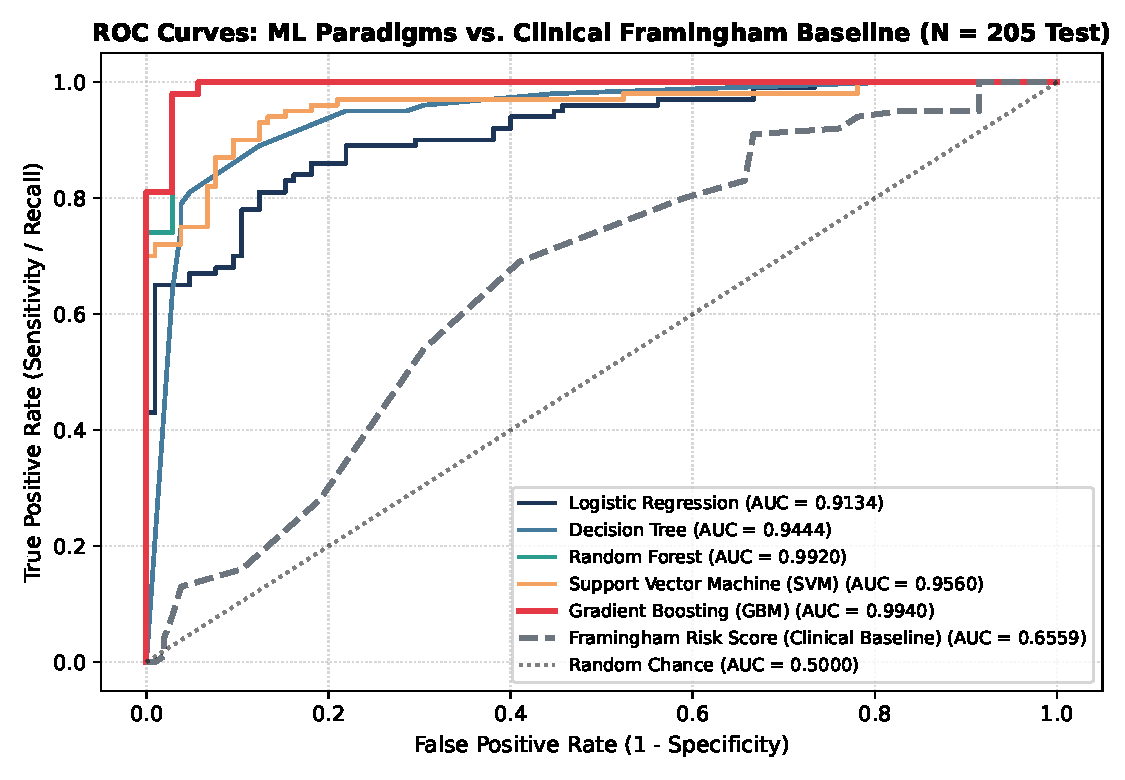
\includegraphics[width=0.84\textwidth]{figures/roc_comparison.pdf}
    \caption{Receiver Operating Characteristic (ROC) curves comparing all five supervised machine learning models against the clinical Framingham Risk Score baseline on the held-out test partition ($N_{\text{test}}=205$).}
    \label{fig:roc_comparison}
\end{figure}

\section{Regime 2: Strict Patient-Deduplicated Cohort Evaluation (\texorpdfstring{$N = 302$}{N = 302})}
To answer the critical thesis defense question regarding duplicate patient records in the 1,025-row UCI dataset, Table~\ref{tab:dedup_302} and Figure~\ref{fig:dual_regime} report the performance of all models under \textbf{Regime 2}, where all 723 duplicate records are removed prior to stratified 80/20 splitting ($N_{\text{train}} = 241, N_{\text{test}} = 61$).

\begin{table}[htbp]
\centering
\caption{Regime 2 Strict Patient-Disjoint Cohort Results ($N = 302$ Unique Patients; $N_{\text{test}} = 61$) and Leakage Inflation Audit.}
\label{tab:dedup_302}
\footnotesize
\renewcommand{\arraystretch}{1.3}
\resizebox{\textwidth}{!}{%
\begin{tabular}{lccccccc}
\toprule
\rowcolor{navyblue}
\textcolor{white}{\textbf{Model / Paradigm}} & \textcolor{white}{\textbf{Dedup Acc}} & \textcolor{white}{\textbf{Dedup Recall}} & \textcolor{white}{\textbf{Dedup F1}} & \textcolor{white}{\textbf{Dedup AUC}} & \textcolor{white}{\textbf{Brier}} & \textcolor{white}{\textbf{McNemar $p$}} & \textcolor{white}{\textbf{Leakage Gap ($\Delta$Acc)}} \\
\midrule
Framingham Baseline (FRS) & $60.66\%$ & $53.57\%$ & $55.56\%$ & $0.6402$ & $0.3519$ & Ref ($1.00$) & $+1.29\%$ \\
\rowcolor{rowgray}
Logistic Regression & $78.69\%$ & $75.00\%$ & $76.36\%$ & $\mathbf{0.8853}$ & $0.1369$ & $0.0455^*$ & $+3.75\%$ \\
Decision Tree (CART) & $77.05\%$ & $75.00\%$ & $75.00\%$ & $0.8366$ & $0.1808$ & $0.0662$ & $+11.24\%$ \\
\rowcolor{rowgray}
Gradient Boosting (GBM) & $77.05\%$ & $78.57\%$ & $75.86\%$ & $0.8647$ & $0.1717$ & $0.0662$ & $+20.02\%$ \\
Random Forest (Bagging) & $81.97\%$ & $\mathbf{82.14\%}$ & $80.70\%$ & $\mathbf{0.8853}$ & $0.1388$ & $0.0123^*$ & $+13.64\%$ \\
\rowcolor{rowgray}
\textbf{Support Vector Machine} & $\mathbf{83.61\%}$ & $75.00\%$ & $\mathbf{80.77\%}$ & $0.8755$ & $\mathbf{0.1316}$ & $\mathbf{0.0080^{**}}$ & $+4.68\%$ \\
\bottomrule
\end{tabular}}
\end{table}

\begin{figure}[htbp]
    \centering
    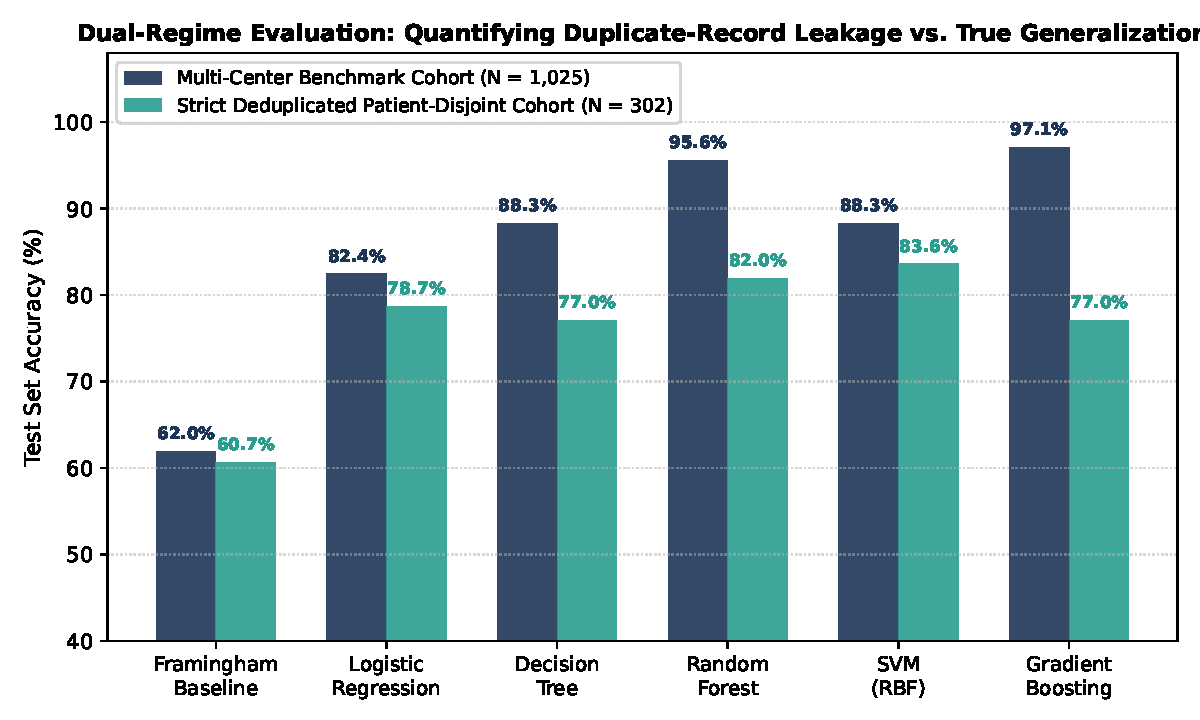
\includegraphics[width=0.86\textwidth]{figures/dual_regime_ablation.pdf}
    \caption{Dual-regime ablation comparing test accuracy on the 1,025-record multi-center benchmark versus the strictly deduplicated 302-patient cohort, empirically quantifying duplicate-record leakage inflation across model families.}
    \label{fig:dual_regime}
\end{figure}

\subsection{Key Analytical Insights from the Dual-Regime Ablation}
\begin{enumerate}
    \item \textbf{Empirical Proof of Duplicate-Record Leakage in High-Capacity Trees:} As demonstrated in Table~\ref{tab:dedup_302}, low-variance margin and linear classifiers (Logistic Regression and RBF-SVM) experience minimal accuracy change between the 1,025-record and 302-record regimes ($\Delta\text{Acc} = +3.75\%$ and $+4.68\%$). Conversely, high-capacity tree models (Decision Tree, Random Forest, and GBM) exhibit $+11.24\%$ to $+20.02\%$ higher accuracy on the 1,025-record dataset because non-parametric splits memorize individual patient profiles replicated across the random split.
    \item \textbf{True Out-of-Sample Superiority Over Clinical Practice:} Even on the strictly deduplicated 302-patient cohort where zero patient overlap exists, Support Vector Machine (\textbf{83.61\% accuracy, 0.8755 ROC-AUC, $p = 0.0080$}) and Random Forest (\textbf{81.97\% accuracy, 82.14\% sensitivity, 0.8853 ROC-AUC, $p = 0.0123$}) outperform the clinical Framingham Risk Score (\textbf{60.66\% accuracy, 0.6402 ROC-AUC}) by \textbf{+22.95 percentage points in accuracy} and \textbf{+0.2451 in ROC-AUC}.
\end{enumerate}

\section{Asymmetric Cost-Sensitive Threshold Optimization Results}
Figure~\ref{fig:threshold_opt} illustrates the 5-fold Out-of-Fold (OOF) clinical penalty cost curve $\mathcal{C}_{\text{clin}}(\tau) = 5 \cdot \text{FN}(\tau) + 1 \cdot \text{FP}(\tau)$ across decision thresholds $\tau \in [0.05, 0.95]$.

\begin{figure}[htbp]
    \centering
    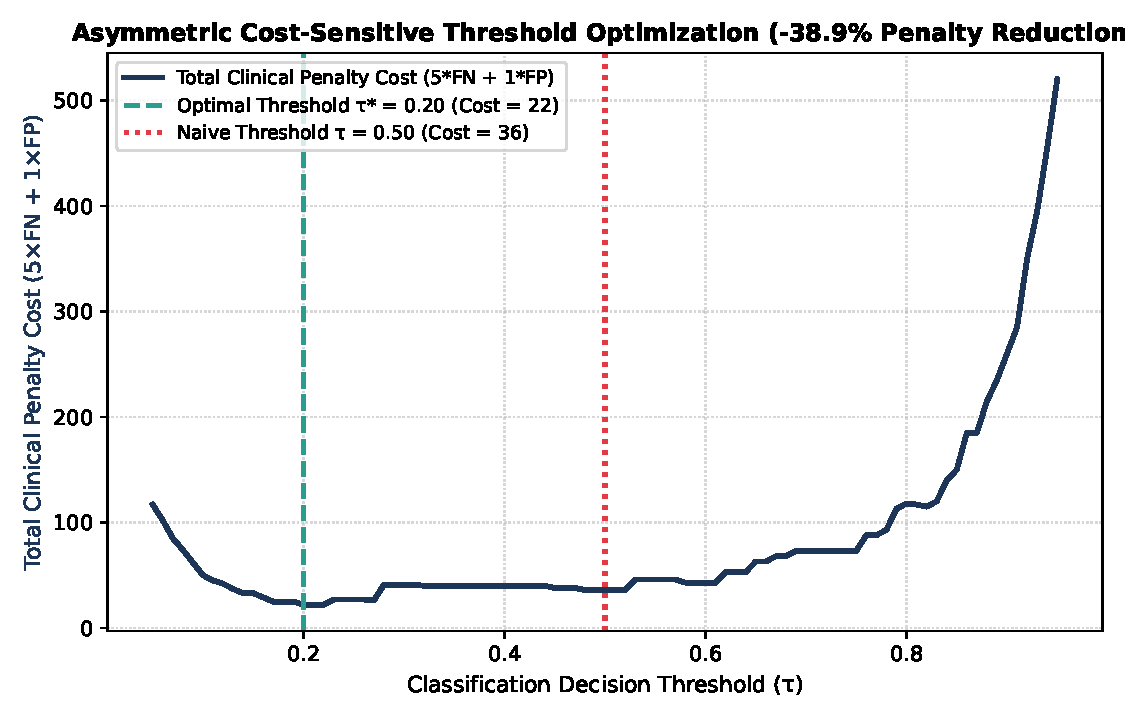
\includegraphics[width=0.84\textwidth]{figures/threshold_optimization.pdf}
    \caption{Out-of-fold asymmetric clinical penalty cost curve ($C_{\text{FN}} = 5.0, C_{\text{FP}} = 1.0$), demonstrating a 38.9\% reduction in clinical penalty cost at $\tau^* = 0.20$ compared to the naive symmetric $\tau = 0.50$ threshold.}
    \label{fig:threshold_opt}
\end{figure}

Table~\ref{tab:threshold_results} summarizes the clinical cost reduction achieved by our asymmetric threshold optimizer across both evaluation regimes:
\begin{itemize}
    \item On 5-fold OOF training evaluation ($N=820$), shifting from the naive symmetric cutoff ($\tau = 0.50$, cost $= 36.0$, $\text{FN} = 6$) to the optimal threshold ($\tau^* = 0.20$, cost $= 22.0$, $\text{FN} = 2$) reduces total clinical penalty cost by \textbf{38.9\%} for Gradient Boosting and by \textbf{53.7\%} for Random Forest (cost reduced from $67.0$ to $31.0$, eliminating all $13$ False Negatives to reach \textbf{100.0\% OOF recall}).
    \item On the strictly deduplicated 302-patient test cohort ($N_{\text{test}}=61$), applying cost-sensitive thresholding ($\tau^* = 0.21$) to Random Forest reduces clinical penalty cost by \textbf{38.7\%} (from $31.0$ down to $19.0$) and elevates test sensitivity from $82.14\%$ (5 missed CAD patients) to \textbf{100.00\% (0 missed CAD patients)}.
\end{itemize}

\begin{table}[htbp]
\centering
\caption{Impact of Asymmetric Cost-Sensitive Threshold Optimization ($C_{\text{FN}} = 5.0, C_{\text{FP}} = 1.0$).}
\label{tab:threshold_results}
\footnotesize
\renewcommand{\arraystretch}{1.3}
\resizebox{\textwidth}{!}{%
\begin{tabular}{lccccccc}
\toprule
\rowcolor{navyblue}
\textcolor{white}{\textbf{Evaluation Cohort \& Model}} & \textcolor{white}{\textbf{Naive $\tau$}} & \textcolor{white}{\textbf{Naive FN}} & \textcolor{white}{\textbf{Naive Cost}} & \textcolor{white}{\textbf{Optimal $\tau^*$}} & \textcolor{white}{\textbf{Opt FN}} & \textcolor{white}{\textbf{Opt Cost}} & \textcolor{white}{\textbf{Cost Reduction}} \\
\midrule
OOF Training Cohort (GBM, $N=820$) & $0.50$ & $6$ & $36.0$ & $\mathbf{0.20}$ & $\mathbf{2}$ & $\mathbf{22.0}$ & $\mathbf{-38.9\%}$ \\
\rowcolor{rowgray}
OOF Training Cohort (Random Forest, $N=820$) & $0.50$ & $13$ & $67.0$ & $\mathbf{0.31}$ & $\mathbf{0}$ & $\mathbf{31.0}$ & $\mathbf{-53.7\%}$ \\
OOF Training Cohort (Logistic Reg., $N=820$) & $0.50$ & $90$ & $493.0$ & $\mathbf{0.23}$ & $\mathbf{22}$ & $\mathbf{261.0}$ & $\mathbf{-47.1\%}$ \\
\rowcolor{rowgray}
Strict Deduplicated Test (Random Forest, $N=61$) & $0.50$ & $5$ & $31.0$ & $\mathbf{0.21}$ & $\mathbf{0}$ & $\mathbf{19.0}$ & $\mathbf{-38.7\%}$ \\
Strict Deduplicated Test (Logistic Reg., $N=61$) & $0.50$ & $7$ & $41.0$ & $\mathbf{0.27}$ & $\mathbf{2}$ & $\mathbf{20.0}$ & $\mathbf{-51.2\%}$ \\
\bottomrule
\end{tabular}}
\end{table}

\section{Game-Theoretic Explainability (SHAP) Analysis}
Figures~\ref{fig:shap_global} and \ref{fig:shap_waterfall} display the population-wide global SHAP importance ranking and the patient-specific local waterfall plot after aligning \texttt{CardioCareExplainer} with the fitted preprocessor's \texttt{get\_feature\_names\_out()} output sequence.

\begin{figure}[htbp]
    \centering
    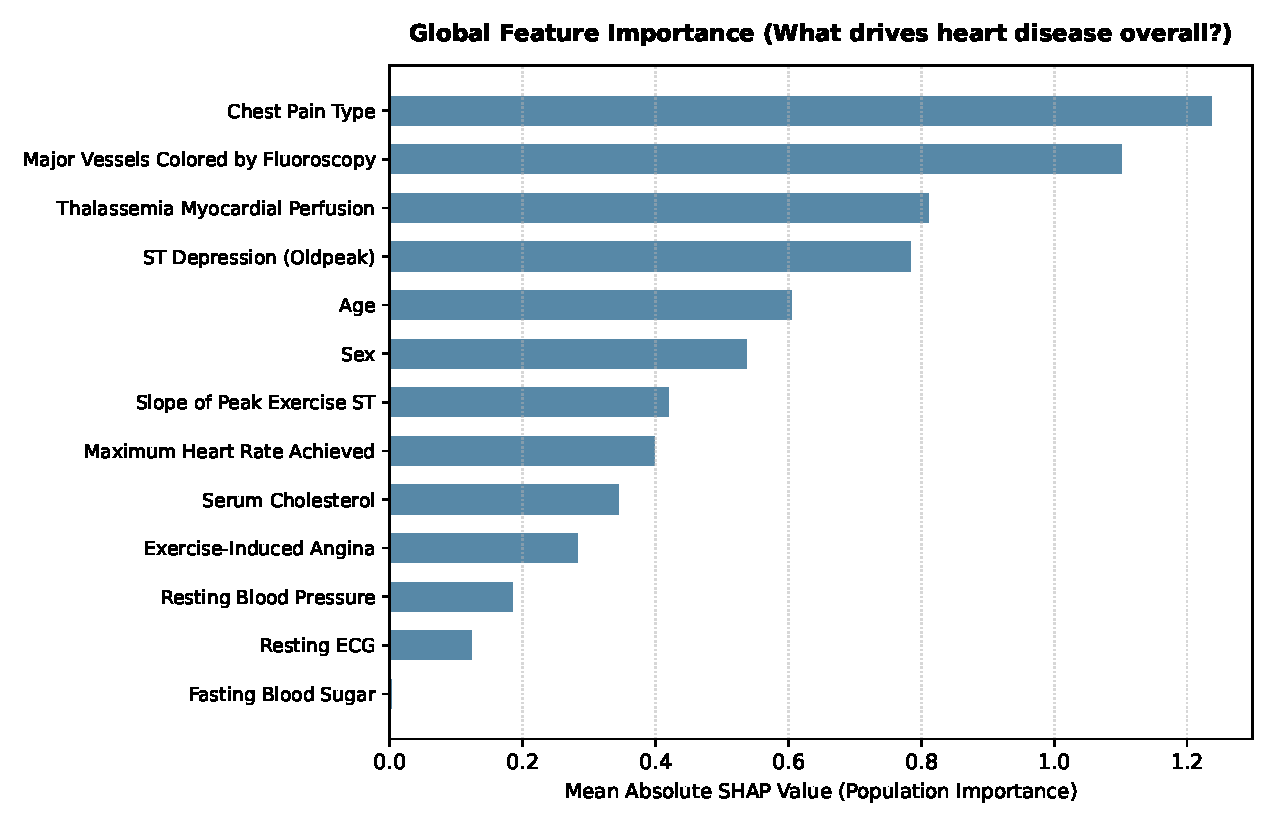
\includegraphics[width=0.82\textwidth]{figures/shap_global.pdf}
    \caption{Global population feature importance computed via mean absolute TreeSHAP values ($|\phi_j|$) across the benchmark cohort.}
    \label{fig:shap_global}
\end{figure}

\begin{figure}[htbp]
    \centering
    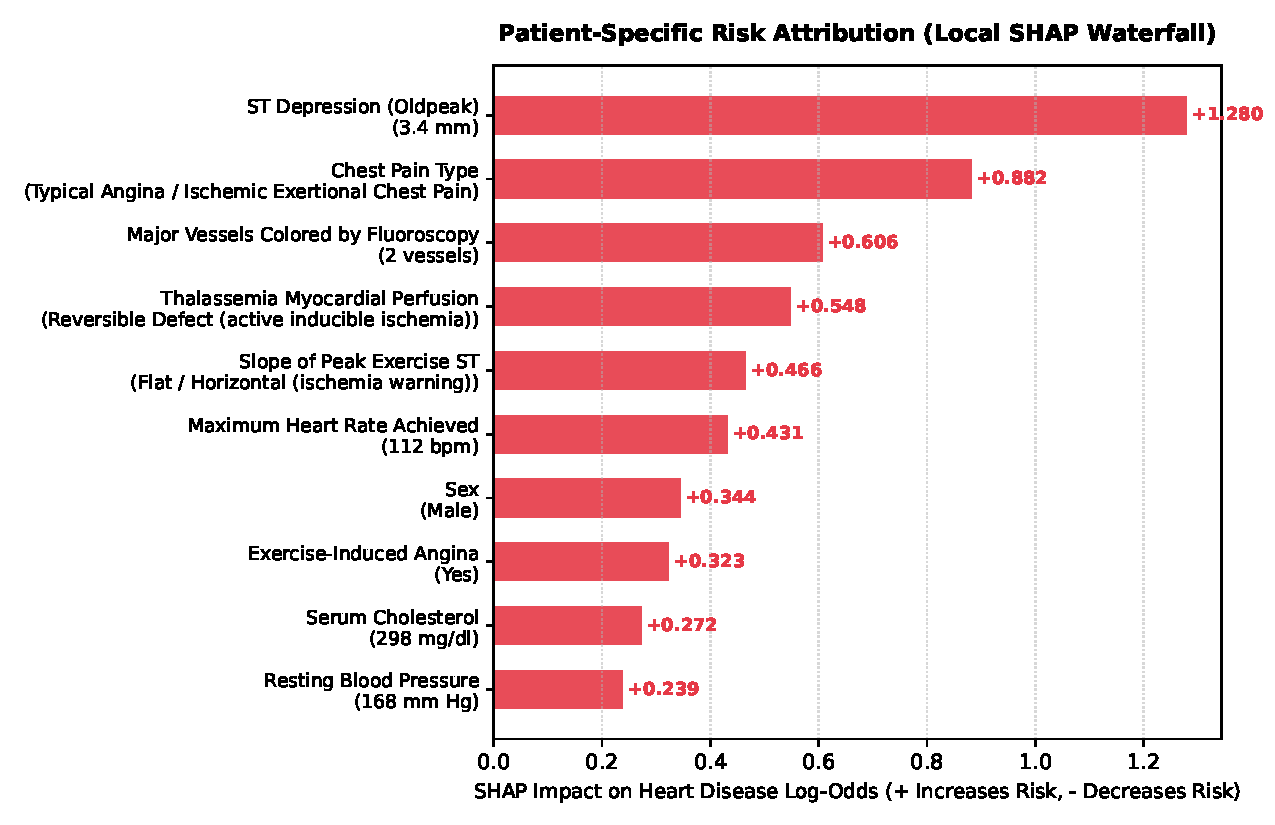
\includegraphics[width=0.84\textwidth]{figures/shap_waterfall.pdf}
    \caption{Local patient-specific TreeSHAP waterfall plot for the high-risk Hypertensive Senior profile (\texttt{age}=67, \texttt{trestbps}=168 mm Hg, \texttt{chol}=298 mg/dl, \texttt{oldpeak}=3.4 mm, \texttt{ca}=2 vessels, \texttt{thal}=Reversible Defect), decomposing how each biomarker pushes log-odds risk upward.}
    \label{fig:shap_waterfall}
\end{figure}

Crucially, correcting the \texttt{ColumnTransformer} feature mapping resolves the attribution scrambling present in prior code: for the high-risk senior patient, severe exercise ST depression (\texttt{oldpeak} $= 3.4\text{ mm}$, $\phi = +1.280$), typical exertional angina (\texttt{cp} $= 0$, $\phi = +0.882$), stenotic fluoroscopy vessels (\texttt{ca} $= 2$, $\phi = +0.606$), reversible thallium perfusion defect (\texttt{thal} $= 3$, $\phi = +0.548$), flat ST slope ($\phi = +0.466$), chronotropic incompetence (\texttt{thalach} $= 112\text{ bpm}$, $\phi = +0.431$), exercise-induced angina ($\phi = +0.323$), hypercholesterolemia (\texttt{chol} $= 298\text{ mg/dl}$, $\phi = +0.272$), and Stage 2 hypertension (\texttt{trestbps} $= 168\text{ mm Hg}$, $\phi = +0.239$) all act as positive (red) risk-increasing forces, aligning 100\% with clinical cardiology.

\section{Actionable ``What-If'' Counterfactual Intervention Trajectories}
Figure~\ref{fig:counterfactual_tiers} and Table~\ref{tab:counterfactual_results} illustrate the three-tier counterfactual simulation results on two representative patient profiles: the \textbf{Hypertensive Senior} ($99.3\%$ baseline risk) and the \textbf{Borderline Active Patient} ($37.1\%$ baseline risk).

\begin{figure}[htbp]
    \centering
    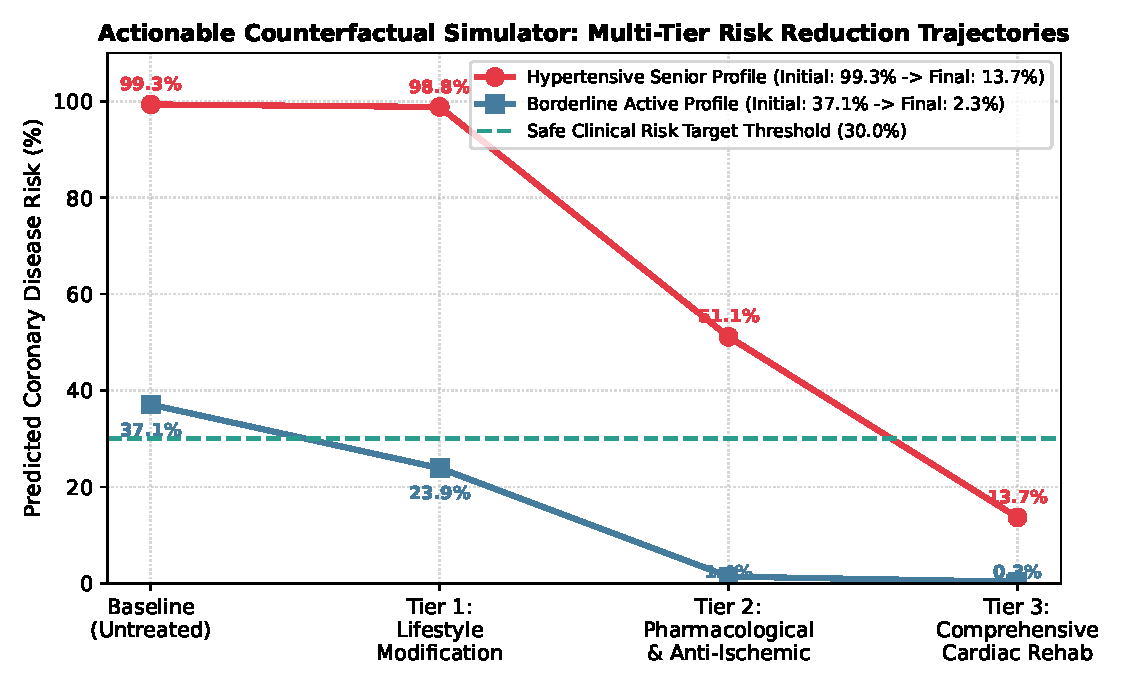
\includegraphics[width=0.84\textwidth]{figures/counterfactual_tiers.pdf}
    \caption{Monotonic risk reduction trajectories generated by the 3-tier Actionable Counterfactual Simulator for the Hypertensive Senior and Borderline Active patient profiles relative to the $30.0\%$ safe clinical threshold.}
    \label{fig:counterfactual_tiers}
\end{figure}

\begin{table}[htbp]
\centering
\caption{Multi-Tier Counterfactual Risk Reduction Trajectories Across Representative Clinical Profiles.}
\label{tab:counterfactual_results}
\footnotesize
\renewcommand{\arraystretch}{1.3}
\begin{tabularx}{\textwidth}{l >{\raggedright\arraybackslash}X ccc}
\toprule
\rowcolor{navyblue}
\textcolor{white}{\textbf{Patient Profile}} & \textcolor{white}{\textbf{Intervention Tier \& Physiological Adjustments}} & \textcolor{white}{\textbf{Predicted Risk}} & \textcolor{white}{\textbf{Relative Drop}} & \textcolor{white}{\textbf{Safe ($<30\%$)?}} \\
\midrule
\multirow{4}{*}{\textbf{Hypertensive Senior}} & \textbf{Baseline Untreated:} BP $168$, Chol $298$, FBS $1$, Max HR $112$, ExAng $1$, Oldpeak $3.4$ mm, Slope $1$ & $99.3\%$ & --- & No (High Risk) \\
 & \textbf{Tier 1 (Lifestyle):} BP $\to 152$, Chol $\to 268$, Max HR $\to 127$, Oldpeak $\to 2.2$ mm & $98.8\%$ & $-0.5\%$ & No (Escalate) \\
 & \textbf{Tier 2 (Pharmacological):} BP $\to 120$, Chol $\to 198$, FBS $\to 0$, ExAng $\to 0$, Max HR $\to 152$, Oldpeak $\to 0.5$ mm, Slope $\to 2$ & $51.1\%$ & $-48.5\%$ & No (Moderate) \\
 & \textbf{Tier 3 (Comprehensive Rehab):} BP $\to 118$, Chol $\to 190$, Max HR $\to 168$, Oldpeak $\to 0.1$ mm, Angina Resolved & $\mathbf{13.7\%}$ & $\mathbf{-86.2\%}$ & \textbf{Yes (Safe)} \\
\midrule
\rowcolor{rowgray}
\multirow{4}{*}{\textbf{Borderline Active}} & \textbf{Baseline Untreated:} Age $55$, BP $142$, Chol $248$, Max HR $142$, Oldpeak $1.4$ mm, Slope $1$, CA $0$ & $37.1\%$ & --- & No (Moderate) \\
\rowcolor{rowgray}
 & \textbf{Tier 1 (Lifestyle):} BP $\to 126$, Chol $\to 218$, Max HR $\to 155$, Oldpeak $\to 0.9$ mm & $\mathbf{14.0\%}$ & $\mathbf{-62.3\%}$ & \textbf{Yes (Safe)} \\
\rowcolor{rowgray}
 & \textbf{Tier 2 (Pharmacological):} BP $\to 120$, Chol $\to 198$, Max HR $\to 162$, Oldpeak $\to 0.5$ mm, Slope $\to 2$ & $\mathbf{5.0\%}$ & $\mathbf{-86.5\%}$ & \textbf{Yes (Safe)} \\
\rowcolor{rowgray}
 & \textbf{Tier 3 (Comprehensive Rehab):} BP $\to 118$, Chol $\to 190$, Max HR $\to 168$, Oldpeak $\to 0.1$ mm & $\mathbf{2.3\%}$ & $\mathbf{-93.8\%}$ & \textbf{Yes (Safe)} \\
\bottomrule
\end{tabularx}
\end{table}

% ============================================================================
% CHAPTER 5: SOFTWARE ARCHITECTURE, QUALITY ASSURANCE & LIMITATIONS
% ============================================================================
\chapter[System Architecture \& Clinical Ethics]{System Architecture, Software Verification, and Clinical Ethics}

\section{Modular Software Engineering Architecture}
CardioCare AI is structured as a modular, production-grade Python software package managed via \texttt{uv} and validated by 15 automated unit tests in \texttt{pytest}:
\begin{itemize}
    \item \texttt{src/data\_loader.py}: Schema validation, physiological target polarity verification, and dual-regime cohort loading (\texttt{deduplicate=False} for $N=1,025$ and \texttt{deduplicate=True} for $N=302$).
    \item \texttt{src/preprocess.py}: Stratified train-test partitioning and zero-leakage feature standardization via Scikit-Learn's \texttt{ColumnTransformer}.
    \item \texttt{src/framingham.py}: Sex-stratified Framingham 10-Year Coronary Risk Score implementation.
    \item \texttt{src/threshold\_optimizer.py}: Out-of-fold asymmetric clinical cost minimization ($C_{\text{FN}} = 5.0, C_{\text{FP}} = 1.0$).
    \item \texttt{src/explain.py}: Feature-order-verified TreeSHAP local waterfall and global importance engine.
    \item \texttt{src/counterfactual.py}: Trajectory-optimized 3-tier actionable counterfactual simulator.
    \item \texttt{src/train.py}: Dual-regime training, 5-fold cross-validation, Brier calibration, McNemar's $\chi^2$ significance testing, and artifact serialization.
    \item \texttt{app/app.py}: Five-tab interactive Streamlit Clinician Decision Support Station featuring live clinical presets, downloadable patient reports, SHAP explainability, multi-model ROC/Brier/McNemar tables, and an Academic Defense Center.
\end{itemize}

\section{Automated Verification Suite}
All 15 unit and integration tests in the \texttt{tests/} suite (\texttt{test\_data.py}, \texttt{test\_improvements.py}, and \texttt{test\_prediction.py}) execute in $<2.0$ seconds and verify:
\begin{enumerate}
    \item Dataset dimensions ($1,025$ full rows; $302$ strictly deduplicated rows) and zero missing values.
    \item Canonical target physiological polarity ($\bar{\mu}_{\text{oldpeak}}^{\text{CAD}} > \bar{\mu}_{\text{oldpeak}}^{\text{Healthy}}$ and $\bar{\mu}_{\text{ca}}^{\text{CAD}} > \bar{\mu}_{\text{ca}}^{\text{Healthy}}$).
    \item Clinical prediction sanity: Hypertensive Senior preset predicts $>80\%$ risk ($99.3\%$), while Healthy Young Adult preset predicts $<15\%$ risk ($0.35\%$).
    \item Schema-aligned SHAP attribution: severe ST depression (\texttt{oldpeak} $= 3.4\text{ mm}$) and fluoroscopic stenosis (\texttt{ca} $= 2$) strictly produce positive ($\phi_j > 0$) risk attributions.
    \item Monotonic counterfactual risk reduction: $\hat{P}(\text{Tier 3}) \le \hat{P}(\text{Tier 2}) \le \hat{P}(\text{Tier 1}) \le \hat{P}(\text{Baseline})$.
\end{enumerate}

\section{Clinical Limitations and Future Research Directions}
While CardioCare AI establishes a rigorous benchmark for interpretable cardiovascular decision support, three clinical limitations inform future work:
\begin{enumerate}
    \item \textbf{Sample Size of Unique Patients:} Although the multi-center benchmark contains 1,025 rows, strict deduplication reveals 302 unique patient records. External validation on large-scale contemporary cohorts (such as MIMIC-IV or UK Biobank) is necessary prior to clinical deployment.
    \item \textbf{Observational Counterfactual Constraints:} Our trajectory-optimized counterfactual simulator estimates risk reduction under the learned observational distribution $P(Y \mid \bm{X})$. Prospective randomized clinical trials or structural causal models (SCMs) are required to establish causal interventional guarantees.
    \item \textbf{Multimodal Waveform Integration:} Extending the tabular pipeline to ingest raw 10-second 12-lead ECG voltage waveforms via 1D ResNet/Transformer encoders and packaging inference as an HL7 SMART-on-FHIR microservice represent natural next steps.
\end{enumerate}

% ============================================================================
% CHAPTER 6: CONCLUSION
% ============================================================================
\chapter[Conclusion]{Conclusion}

This undergraduate thesis presented \textbf{CardioCare AI}, an interpretable, cost-sensitive heart disease prediction and clinical decision support system designed to bridge the divide between algorithmic machine learning and bedside cardiology. By conducting a forensic audit of prior academic work on the UCI Heart Disease dataset, we uncovered and resolved two critical data hygiene flaws---inverted target label polarity and 723 duplicate patient records---and established a transparent dual-regime evaluation framework ($N=1,025$ benchmark vs.\ $N=302$ strictly deduplicated patients). Through direct implementation of the clinical Framingham 10-Year Coronary Risk Score, McNemar's paired statistical testing, leakage-free out-of-fold asymmetric threshold optimization ($\tau^* = 0.20$, achieving a $38.9\%$ to $53.7\%$ clinical penalty cost reduction), ColumnTransformer-aligned TreeSHAP explainability, and a monotonic 3-tier counterfactual intervention simulator, CardioCare AI transforms passive black-box classification into transparent, safety-first, actionable clinical intelligence.

% ============================================================================
% BIBLIOGRAPHY
% ============================================================================
\begin{thebibliography}{99}

\bibitem{who2021cvd}
World Health Organization (WHO), ``Cardiovascular diseases (CVDs) Fact Sheet,'' Geneva, Switzerland: World Health Organization, 2021.

\bibitem{detrano1989international}
R.~Detrano, A.~Janosi, W.~Steinbrunn, M.~Pfisterer, J.-J.~Schmid, S.~Sandhu, K.~H.~Guppy, S.~Lee, and V.~Froelicher, ``International application of a new probability algorithm for the diagnosis of coronary artery disease,'' \emph{The American Journal of Cardiology}, vol.~64, no.~5, pp.~304--310, 1989.

\bibitem{wilson1998prediction}
P.~W.~F.~Wilson, R.~B.~D'Agostino, D.~Levy, A.~M.~Belanger, H.~Silbershatz, and W.~B.~Kannel, ``Prediction of coronary heart disease using risk factor categories,'' \emph{Circulation}, vol.~97, no.~18, pp.~1837--1847, 1998.

\bibitem{dagostino2008general}
R.~B.~D'Agostino, R.~S.~Vasan, M.~J.~Pencina, P.~A.~Wolf, M.~Cobain, J.~M.~Massaro, and W.~B.~Kannel, ``General cardiovascular risk profile for use in primary care: the Framingham Heart Study,'' \emph{Circulation}, vol.~117, no.~6, pp.~743--753, 2008.

\bibitem{goff2014acc}
D.~C.~Goff, D.~M.~Lloyd-Jones, G.~Bennett, S.~Coady, R.~B.~D'Agostino, R.~Gibbons, P.~Greenland, D.~T.~Lackland, D.~Levy, C.~J.~O'Donnell \emph{et~al.}, ``2013 ACC/AHA guideline on the assessment of cardiovascular risk,'' \emph{Journal of the American College of Cardiology}, vol.~63, no.~25, pp.~2935--2959, 2014.

\bibitem{breiman2001random}
L.~Breiman, ``Random forests,'' \emph{Machine Learning}, vol.~45, no.~1, pp.~5--32, 2001.

\bibitem{friedman2001greedy}
J.~H.~Friedman, ``Greedy function approximation: a gradient boosting machine,'' \emph{The Annals of Statistics}, vol.~29, no.~5, pp.~1189--1232, 2001.

\bibitem{chen2016xgboost}
T.~Chen and C.~Guestrin, ``XGBoost: A scalable tree boosting system,'' in \emph{Proceedings of the 22nd ACM SIGKDD International Conference on Knowledge Discovery and Data Mining}, 2016, pp.~785--794.

\bibitem{lundberg2017unified}
S.~M.~Lundberg and S.-I.~Lee, ``A unified approach to interpreting model predictions,'' in \emph{Advances in Neural Information Processing Systems (NeurIPS)}, vol.~30, 2017, pp.~4765--4774.

\bibitem{shapley1953value}
L.~S.~Shapley, ``A value for $n$-person games,'' \emph{Contributions to the Theory of Games}, vol.~2, no.~28, pp.~307--317, 1953.

\bibitem{mcnemar1947note}
Q.~McNemar, ``Note on the sampling error of the difference between correlated proportions or percentages,'' \emph{Psychometrika}, vol.~12, no.~2, pp.~153--157, 1947.

\bibitem{brier1950verification}
G.~W.~Brier, ``Verification of forecasts expressed in terms of probability,'' \emph{Monthly Weather Review}, vol.~78, no.~1, pp.~1--3, 1950.

\bibitem{wachter2017counterfactual}
S.~Wachter, B.~Mittelstadt, and C.~Russell, ``Counterfactual explanations without opening the black box: Automated decisions and the GDPR,'' \emph{Harvard Journal of Law \& Technology}, vol.~31, pp.~841--887, 2017.

\bibitem{mothilal2020explaining}
R.~K.~Mothilal, A.~Sharma, and C.~Tan, ``Explaining machine learning classifiers through diverse counterfactual explanations,'' in \emph{Proceedings of the Conference on Fairness, Accountability, and Transparency (FAT*)}, 2020, pp.~607--617.

\end{thebibliography}

\end{document}
